\documentclass[12pt, a4paper]{article}

% --- Essential Packages ---
\usepackage{cite} 
\usepackage[utf8]{inputenc}
\usepackage[margin=1in]{geometry}   % Standard 1-inch margins
\usepackage{graphicx}               % REQUIRED for \includegraphics and images
\usepackage{amsmath, amssymb}       % Math formatting
\usepackage{booktabs}               % Professional tables
\usepackage{hyperref}               % Interactive links and bookmarks
\usepackage{xcolor}                 % Enables color commands and standard color names
\usepackage{tabularx}               % Enables tabularx environment and X columns
\usepackage{array}                  % Advanced table array handling
\usepackage{mdframed}               % Creates clean bordered boxes for prompt blocks
\usepackage{enumitem}               % Advanced list formatting
\usepackage{makecell}               % Allows manual line breaks \\ inside table headers
\usepackage{booktabs}               % Professional tables
\usepackage{tabularx}               % Enables tabularx environment
\usepackage{xltabular}             % Allows multi-page tables with X columns
\usepackage{float}

% --- Hyperlink Formatting ---
\hypersetup{
    colorlinks=true,
    linkcolor=blue!80!black,  % Colors Figure/Table/Section refs a deep blue
    citecolor=green!50!black, % Colors bibliography citations (\cite)
    urlcolor=blue             % Colors external web links
}


\begin{document}

% ==============================================================================
% COVER PAGE
% ==============================================================================
\begin{titlepage}
    \centering
    \vspace*{0.5cm}
    
    % Course Title
    {\Large \textbf{Module ()}}\\[0.3cm]
    {\large \textbf{Assessment Title}}\\[0.1cm]
    
    % Author & Candidate Info
    \begin{tabular}{r l}
        \textbf{Author:} & Luke Birkett \\
        \textbf{Candidate ID:} & 22411525 \\
        \textbf{Word Count:} &  \\
    \end{tabular}\\[0.5cm]
    
    % Abstract Section
    \begin{minipage}{0.92\textwidth}
        \small
        \textbf{\abstractname}\\[0.3em]
        This report 
    \end{minipage}\\[1cm]
    
    % AI Usage Statement Section
    \begin{minipage}{0.92\textwidth}
        \small
        \textbf{AI Usage Statement}\\[0.3em]
        In accordance with university guidelines, generative AI tools---specifically Gemini---were used strictly in an assistive role throughout the preparation of this report. AI was deployed as a refining and coding partner to improve report readability through spell-checking, grammar refinement, and copywriting iteration. It was also utilized to convert technical functions and explanations into \LaTeX{} equations and to generate inline code comments. AI was not used to generate any original content. AI was not used derive insights or analyse results. All methodologies, analysis, conclusions, and interpretations represent my own independent work based on learning from this module. All AI-assisted text and code were carefully reviewed, edited, and approved prior to submission, and I take full responsibility for all submitted material.
    \end{minipage}

    \vfill
    
\end{titlepage}

% ==============================================================================
% FRONT MATTER: CONTENTS & LISTS
% ==============================================================================
\newpage
\pagenumbering{roman}

% 1. Table of Contents
\tableofcontents
\newpage

% 2. List of Tables
\newpage
\listoftables
\vspace{1cm}

% 3. List of Figures
\newpage
\listoffigures
\vspace{1cm}

% ==============================================================================
% START OF REPORT
% ==============================================================================

\newpage
\pagenumbering{arabic}

% ==============================================================================
% 1. INTRODUCTION
% ==============================================================================
\section{Introduction}
\label{sec:introduction}

\subsection{Network Science Introduction}
\label{subsec:net_sci_intro}
Network science offers a versatile framework for examining complex systems. By representing real-world interactions as formal graphs of nodes and links, it enables the evaluation of system-wide topology and dynamics. Its applications range from identifying key central entities in social systems \cite{wasserman1994, newman2001} and detecting functional communities \cite{fortunato2010} to modeling biological cascades \cite{pastor2001} and assessing structural robustness \cite{lusseau2003emergent, newman2003structure}. By shifting away from isolationist views of individual components, network science reveals the emergent organizational principles and collective behaviors governing modern complex systems.

\subsection{Why Apply Network Science to Football}
\label{subsec:why_network_football}
This report focuses on applying network science to sport \cite{araujo2006ecological}, specifically football \cite{duch2010quantifying}. Traditional football analytics relies primarily on isolated, terminal metrics such as completed passes, goals scored, or advanced modeled metrics like Expected Goals (xG) \cite{pollard1997xg} to quantify performance. However, evaluating players in isolation is fundamentally limited because football operates as a complex adaptive system \cite{buldu2019}. Team success cannot be understood through individual actions alone, instead it emerges from continuous collective interactions, dynamic spatial relationships, and tactical organization \cite{gama2026stoch}.

\subsection{How Apply Network Science to Football}
\label{subsec:how_network_football}
Applying network science requires decomposing a complex system into discrete nodes and directed edges. In football, outfield teammates are modeled as nodes ($N = 11$), while relational interactions between them form the connecting edges. Completed passes provide a pragmatic, objective event stream encoding tactical intent and spatial structure. Representing players as nodes and directed pass volumes as weighted edges forms the foundation of the PassMap paradigm \cite{buldu2018}. A comprehensive explanation of this paradigm is detailed and visualized in Section~\ref{sec:paradigms}.

\subsection{The Null Baseline Problem and Project Scope}
\label{subsec:null_problem_scope}
Evaluating raw football network metrics in isolation offers limited analytical value, as network properties are shaped by underlying topological and spatial constraints. Without baseline distributions, analysts cannot separate deliberate tactical execution from stochastic match noise. Constructing valid null models in football requires reconciling randomized generative processes with physical pitch geometry, spatial proximity, and positional roles. Responding to explicit calls for null models in football from contemporary literature \cite{gama2026stoch}, this project develops a 1st-order Spatial Markovian null framework to generate domain-aware reference ensembles, establishing a robust statistical baseline for tactical evaluation.

% ==============================================================================
% 2. DATA
% ==============================================================================
\newpage
\section{Data}
\label{sec:data}

The dataset used comes from StatsBomb Open-Source event data from the 2023/2024 FA Women's Super League (\texttt{competition\_id: 37}, \texttt{season\_id: 281}). Focusing on women's football directly addresses literature deficits regarding the overreliance on men's samples and the systemic underrepresentation of longitudinal women's datasets \cite{alves2025review, gama2026stoch}.

Raw non-relational event logs are engineered into directed, weighted adjacency matrices $A_{ij}$. For our PassMap framework, we isolate completed passes using four attributes:
\begin{itemize}[leftmargin=*, itemsep=3pt, parsep=0pt]
    \item Passer (source node $i$) + Role
    \item Recipient (target node $j$) + Role
    \item Origin $(x_1, y_1)$
    \item Destination $(x_2, y_2)$
\end{itemize}

StatsBomb's $120 \times 80$ yard pitch coordinates are rescaled to a normalized $100 \times 100$ grid to standardize across varying venue dimensions \cite{buldu2019}. Figure~\ref{fig:raw_passes} illustrates this raw pass data before network transformation.

\begin{figure}[htbp]
    \centering
    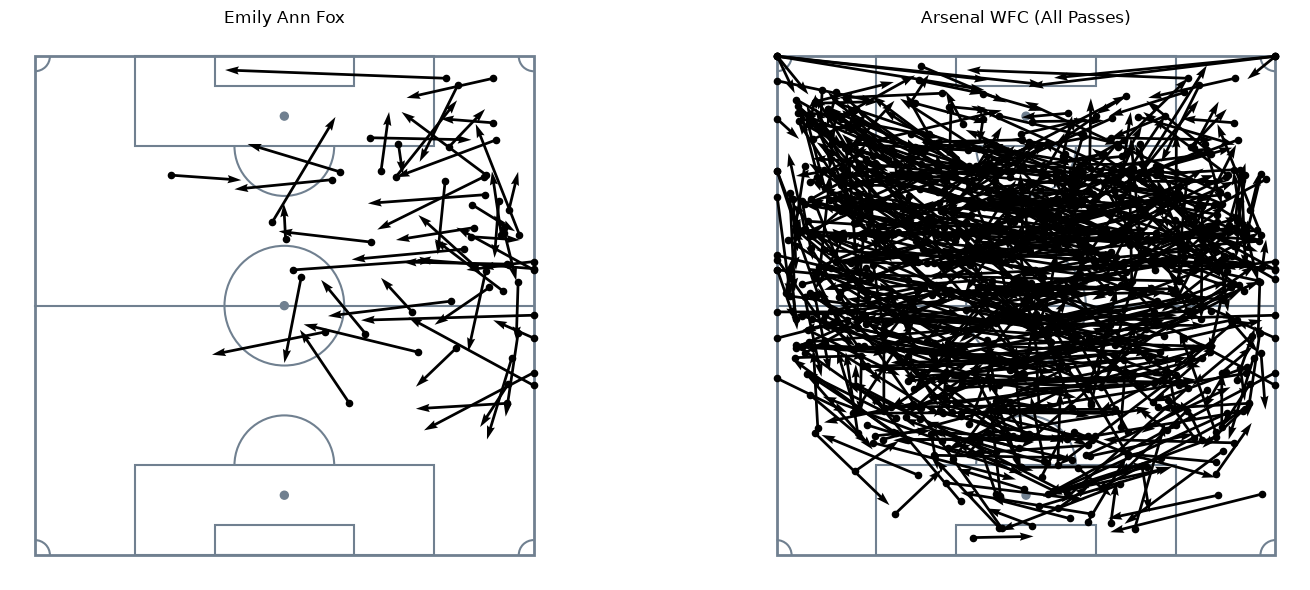
\includegraphics[width=0.9\textwidth]{figures/raw_passes.png}
    \caption{Raw Pass Plotting: Individual Player vs. Whole Team.}
    \label{fig:raw_passes}
\end{figure}

\begin{table}[htbp]
    \centering
    \caption{Summary of Dataset Statistics (WSL 2023/2024)}
    \label{tab:dataset_stats}
    \begin{tabularx}{\textwidth}{X r}
        \toprule
        \textbf{Metric Category} & \textbf{Dataset Statistic} \\
        \midrule
        \textbf{Competition/Season} & FA Women's Super League (WSL) $2023/2024$ \\
        \textbf{Total Matches} & 132 \\
        \textbf{Total Team Networks} & 264 \\
        \textbf{Total Season Passes Recorded} & 89,781 \\
        \textbf{Match-Team Mean Passes} & 399 (Range: 120--847) \\
        \bottomrule
    \end{tabularx}
\end{table}

% ==============================================================================
% 3. PASSING NETWORK PARADIGMS
% ==============================================================================
\newpage
\section{Passing Network Paradigms}
\label{sec:paradigms}

Passes are modeled using the PassMap paradigm popularized by Buld{\'u} et al. \cite{buldu2019} and represented as a directed, weighted graph $G = (V, E, W)$ where edges ($E$) denote completed passes and edge weights ($W$) quantify pass volume between nodes during a match.

While literature outlines alternative formulations---such as purely geographic Pitch-Location networks or high-density composite Player-Pitch networks \cite{narizuka2014statistical, buldu2018}---this project focuses exclusively on the Player PassMap paradigm. Here, the node set corresponds directly to the eleven on-pitch players ($|V| = 11$) which are enriched with identities and mean spatial $(x, y)$ coordinates as node attributes. Most network properties are invariant to the node coordinates but allocating them significantly enhances visual interpretability. To preserve an $N = 11$ network structure despite match substitutions $N > 11$, we model only the 11 players with the highest minutes played. 

Player Networks represent the standard approach in football analytics \cite{duch2010quantifying, alves2025review, gama2026review}. They maintain intuitive alignment with real-world tactical play while avoiding artificial spatial discretization steps that lack consensus standards \cite{narizuka2014statistical, arriaza2018applying}. 

As shown in Figure~\ref{fig:passmaps}, plotting these networks either directly overlaying pitch boundaries or in a frameless spatial layout preserves structural clarity while surfacing emergent team interactions.

\begin{figure}[htbp]
    \centering
    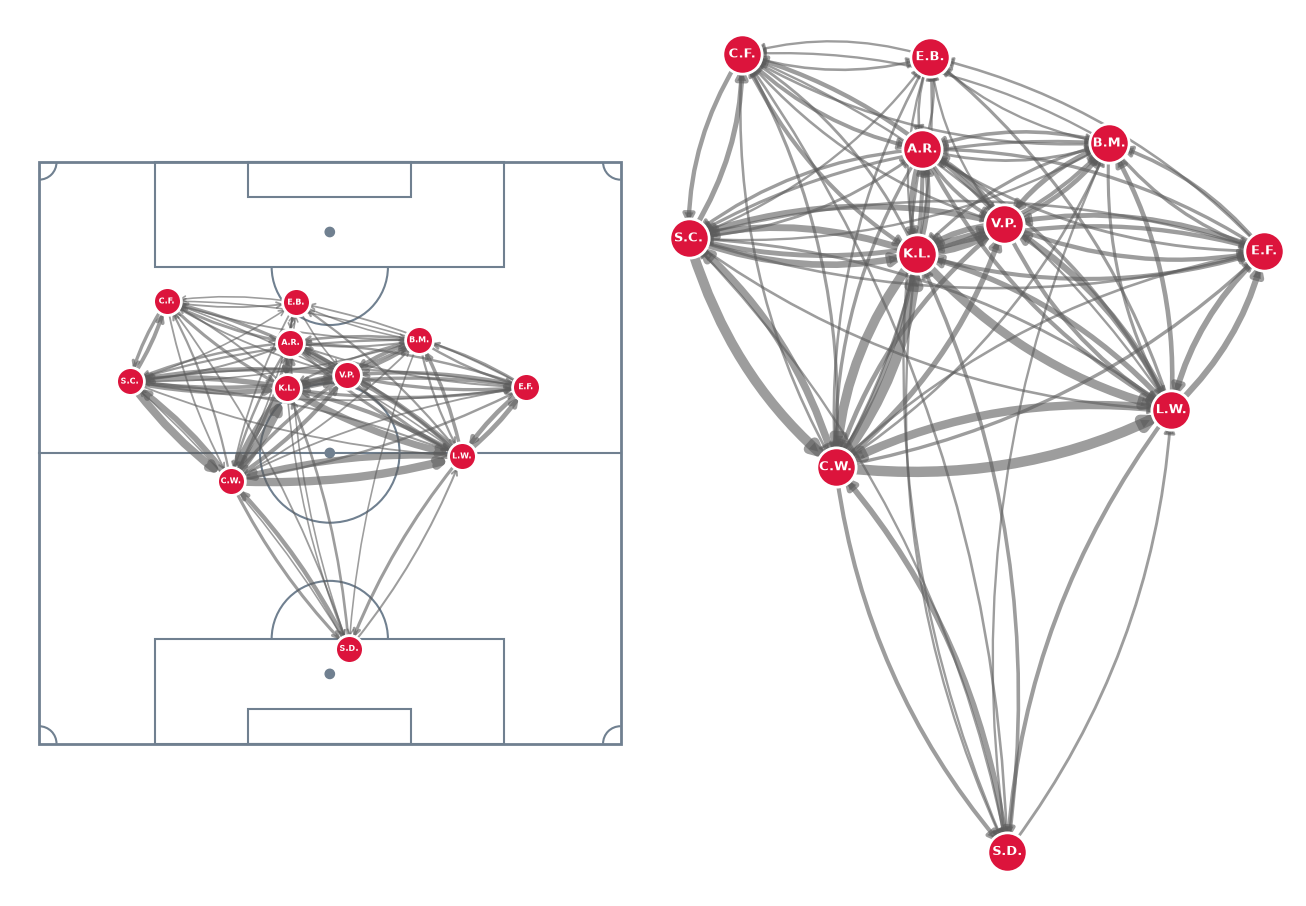
\includegraphics[width=0.9\textwidth]{figures/passmap_examples.png}
    \caption{Pitch-overlay PassMap vs. frameless spatial PassMap.}
    \label{fig:passmaps}
\end{figure}

% ==============================================================================
% 4. FOOTBALL NETWORK METRICS
% ==============================================================================
\newpage
\section{Football Network Metrics}
\label{sec:metrics}

Applying network science to football allows us to decompose and analyze system tactics through mathematical properties \cite{pena2012network}. Gama et al. \cite{gama2026stoch} provide a comprehensive translation of network properties into footballing interpretations (\hyperref[app:network_metrics_taxonomy]{Appendix~\ref{app:network_metrics_taxonomy}}).

To demonstrate the utility of network analysis, we compose a suite of metrics which we apply to the high-volume outlier network from Figure~\ref{fig:passmaps} (Arsenal WFC), a match which recorded the season's highest pass volume for a single team. This is a particularly compelling instance to evaluate in order to determine whether the observed topological properties represent deliberate tactical execution or are merely emergent artifacts of extreme pass volume.

\subsection{Metric Suite}
\label{subsec:metric_suite}
To systematically map network properties to tactical concepts, analysis is categorized into three structural scales: Macro, Meso, and Micro \cite{alves2025review, gama2026review}. This project targets a core suite of metrics across these scales to balance theoretical rigor with clear domain interpretation.

Macro-scale analysis evaluates global team cohesion, structural fluidity, and spatial dominance across the entire network \cite{watts1998collective, cintia2015network}. We examine overall connectivity and structural skew through Unweighted Degree Heterogeneity ($CV_k$) and Team Node Volume Variance ($\text{Var}(s_{\text{tot}})$), alongside multi-step cohesion using the Global Average Shortest Path ($d$).

Meso-scale analysis assesses localized sub-graphs and multi-player combinational passing channels \cite{pena2015can}. We quantify passing triangle strength and progressive build-up chains using Transitive Triad Intensity ($I_{\text{transitive}}$), ranking clusters by their weakest link ($W_{\text{min}}$).

Micro-scale analysis evaluates individual player workload, system asymmetry, and possession control \cite{pena2012network, buldu2019}. We measure pitch control through Betweenness Centrality ($g(i)$) based on inverted topological distance ($l_{ij} = 1/w_{ij}$).

\subsection{Degree-Based Metrics}
\label{subsec:degree_metrics}
Degree-based metrics evaluate system topology using direct, 1-hop connections, avoiding global path-traversal costs to provide a computationally efficient proxy for tactical systems and pass distribution \cite{narizuka2014statistical}.

Evaluating unweighted degree across our high-volume sample network yields a Mean Unweighted Degree of $\langle k \rangle = 16.18$, indicating high overall connectivity out of a theoretical maximum bound of 20. The low Coefficient of Variation ($CV_k = 0.1724$) and near-identical Normalized Second Moment ($\langle k^2 \rangle / \langle k \rangle = 16.66$) confirm that the existence of passing lanes is widely distributed across squad positions, eliminating absolute topological bottlenecks.

However, introducing weighted metrics highlights a critical tactical distinction between structural availability and actual flow of passes. The high Team Node Volume Variance ($\text{Var}(s_{\text{tot}}) = 5,681.90$) reveals that while available passing channels are widespread, pass workload is heavily skewed through specific players.

\newpage
\subsection{Average Shortest Path ($d$)}
\label{subsec:asp}
Edge weights ($w_{ij}$) reflect completed passes from player $i$ to player $j$. In football, pass volume is a stronger indicator of connectivity than physical distance, so edge weights are inverted to derive a topological distance:
\begin{equation}
    l_{ij} = \frac{1}{w_{ij}}
\end{equation}

This transformation ensures high-frequency passing channels yield lower topological resistance. Using Dijkstra’s algorithm, the shortest path ($p_{ij}$) between any pair of players represents the minimal cumulative cost required to move possession through the network.

The macro-level baseline of a team's passing structure is established by the global average shortest path length ($d$), defined as:
\begin{equation}
    d = \frac{1}{N(N-1)} \sum_{i \neq j} p_{ij}
\end{equation}

Arsenal WFC demonstrates strong circulation efficiency with a global path length of $d = 0.1884$, meaning the average cost to route possession between any two arbitrary players is less than $0.20$. Low path length ($d$) is a prerequisite of the Small-World phenomenon \cite{watts1998collective}. In football, it indicates an integrated network capable of rapid ball circulation. However, evaluating $d = 0.1884$ in isolation is arbitrary and cannot confirm tactical superiority. This requires statistical benchmarking against domain-aware null models.

\begin{table}[htbp]
    \centering
    \caption{Highest Pass Match Network Macro Degree Metrics}
    \label{tab:degree_metrics}
    \begin{tabularx}{\textwidth}{X r}
        \toprule
        \textbf{Metric} & \textbf{Value} \\
        \midrule
        \textbf{Team Node Volume Variance} $\text{Var}(s_{\text{tot}})$ & 5681.9008 \\
        \textbf{Mean Unweighted Degree} $\langle k \rangle$ & 16.1818 \\
        \textbf{Degree Variance} $\text{Var}(k)$ & 7.7851 \\
        \textbf{Degree Standard Deviation} $\sigma_k$ & 2.7902 \\
        \textbf{Second Moment} $\langle k^2 \rangle$ & 269.6364 \\
        \textbf{Coefficient of Variation} $CV_k$ & 0.1724 \\
        \textbf{Normalized Second Moment} $\langle k^2 \rangle / \langle k \rangle$ & 16.6629 \\
        \bottomrule
    \end{tabularx}
\end{table}

\newpage
\subsection{Betweenness Centrality ($g(i)$)}
\label{subsec:betweenness}
To evaluate which players act as essential routing hubs, Betweenness Centrality ($g(i)$) is analyzed. Moving beyond volume, betweenness measures the proportion of a network's shortest topological paths ($l_{ij} = 1/w_{ij}$) traversing a given node, identifying possession flow:
\begin{equation}
    g(i) = \sum_{s \neq i \neq t} \frac{\sigma_{st}(i)}{\sigma_{st}}
\end{equation}
where $\sigma_{st}$ represents the total shortest paths between source player $s$ and target player $t$, and $\sigma_{st}(i)$ is the number of those paths passing through player $i$.

Providing deeper inference than 1-hop volume metrics, high scores denote players upon whom phase transitions depend, whereas scores of $0.0000$ mark peripheral endpoints whose exclusion does not disrupt global network routing.

In our sample network, central defenders Lotte Wubben-Moy ($g(i) = 0.3222$) and Leah Williamson ($g(i) = 0.3000$) record the highest centrality, acting as primary structural pivots during recycling and build-up phases---a finding consistent with contemporary football network literature \cite{alves2025review}.

Interpreting betweenness in football requires a key domain-specific nuance. In classic network science, high betweenness denotes a central bottleneck bridge. In football, topological distance allows a physically longer route to represent an easier, low-resistance option. Therefore, deep-lying central defenders can exhibit high centrality by recycling and re-routing phases of play.

Midfielders Kim Little ($0.1778$) and Victoria Pelova ($0.1389$) follow as traditional vertically bridging central players. Conversely, front-line attackers and the goalkeeper register scores of $0.0000$, confirming their roles as terminal nodes rather than network bridges.

\begin{figure}[htbp]
    \centering
    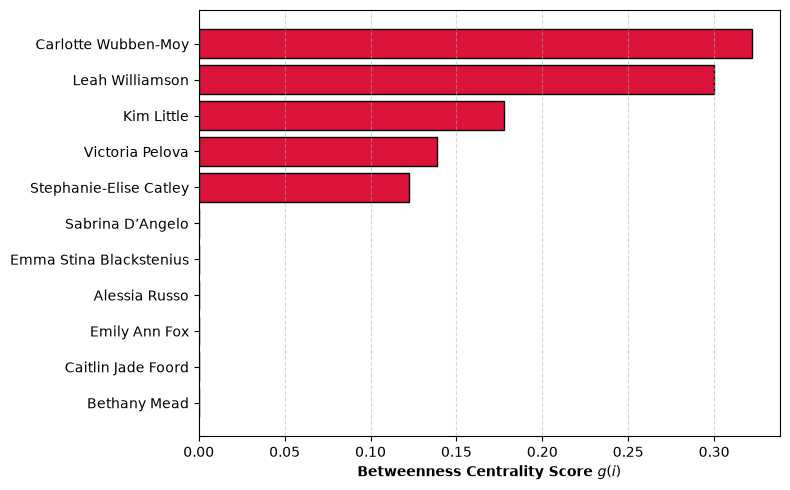
\includegraphics[width=0.85\textwidth]{figures/bet_bar_chart.png}
    \caption{Highest Pass Match Betweenness Centrality $g(i)$ distribution (\hyperref[app:sample_betweenness_scores]{Appendix~\ref{app:sample_betweenness_scores}}).}
    \label{fig:betweenness_bar}
\end{figure}

\newpage
\subsection{Clustering: Transitive Triads ($I_{\text{transitive}}$)}
\label{subsec:clustering}
To evaluate localized spatial cohesiveness and combinational dynamics across the squad, we analyze Transitive Triad Intensity ($I_{\text{transitive}}$). Standard unweighted clustering coefficients can be misleading in football because they treat all connections equally regardless of direction or volume. Transitive triads explicitly isolate progressive wall-passes and multi-option positional triangles ($A \to B \to C$ with $A \to C$), omitting backward cyclic loops ($A \to B \to C \to A$) that rarely denote tactical progression.

As passing networks are weighted by pass volume, a triad's strength is constrained by its weakest link:
\begin{equation}
    W_{\text{min}} = \min(W_{AB}, W_{BC}, W_{AC})
\end{equation}

By ranking individual triads by the strength of their weakest link ($W_{\text{min}}$), we isolate the specific three-player passing circuits where Arsenal most frequently established progressive combination relationships (\hyperref[app:empirical_triads]{Appendix~\ref{app:empirical_triads}}).

The highest-capacity triad (Kim Little, Lotte Wubben-Moy, Leah Williamson, $W_{\text{min}} = 116.0$) highlights a resilient central triangle anchoring initial build-up out of defense, while left-sided loops involving Steph Catley account for three of the top six most active circuits, indicating asymmetric possessional competency. Overlaying these top-capacity transitive triads onto the PassMap (Figure~\ref{fig:triad_plot}) converts a dense network into identifiable passing triangles.

\begin{figure}[H]
    \centering
    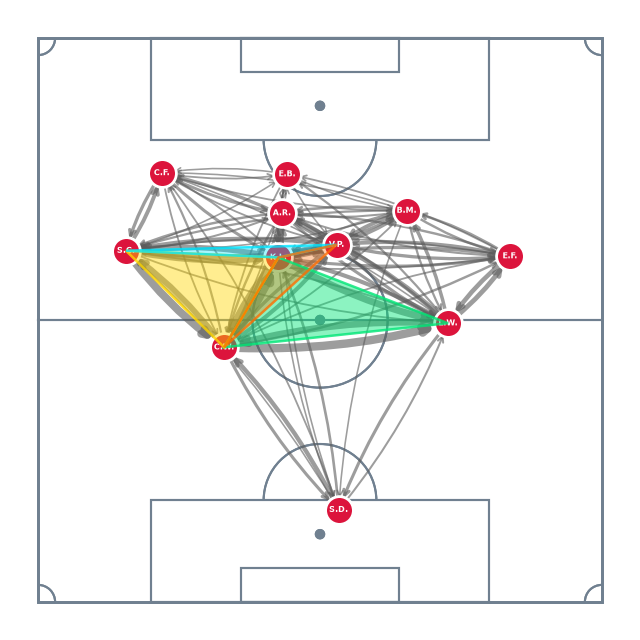
\includegraphics[height=0.52\textheight, keepaspectratio]{figures/triad_plot.png}
    \caption{Highest Pass Match Top Transitive Triads Overlay.}
    \label{fig:triad_plot}
\end{figure}

% ==============================================================================
% 5. EMPIRICAL BASELINE CONSTRAINTS
% ==============================================================================
\newpage
\section{Empirical Baseline Constraints}
\label{sec:empirical_constraints}

Tactical network analysis generally requires benchmarking against a league-wide baseline. Evaluating global average shortest path lengths ($d$) across all season matches places our sample network ($d = 0.1884$) in the top 3.41\% of league efficiency, approaching the season minimum ($0.1748$) from a league mean (std) $0.3521 \pm 0.1263$ .

However, networks properties are heavily dictated by edge volume and spatial topology and this match was selected as it is the league's peak pass volume outlier. Binning the pass data  exposes severe data-sparsity constraints for empirical comparisons.  Bins of 100-pass increments show that the 200--299 pass range holds $40.2\%$ of league matches (94 of 234), whereas higher volume tiers drop off rapidly: 500--599: 14 matches, 600--699: 8, and 700--799: 1, exclusively our single sample match (\hyperref[fig:pass_histogram]{Figure~\ref{fig:pass_histogram}}).

Benchmarking also requires controlling for tactical formation to normalize network topology. Segmenting even the largest pass-volume bin across the 11 recorded formations reduces the primary setup (4-2-3-1) to just 29 instances and 3 formation categories carry a single instance (\hyperref[app:positional_taxonomy]{Appendix~\ref{app:positional_taxonomy}}). Dual filtering for pass volume and formation severely restricts sample sizes, preventing robust statistical evaluation. Despite using a comprehensive season-wide dataset, that is large by literature standards \cite{gama2026stoch}, these sparsity constraints necessitate generating null models to benchmark analysis.

\begin{figure}[htbp]
    \centering
    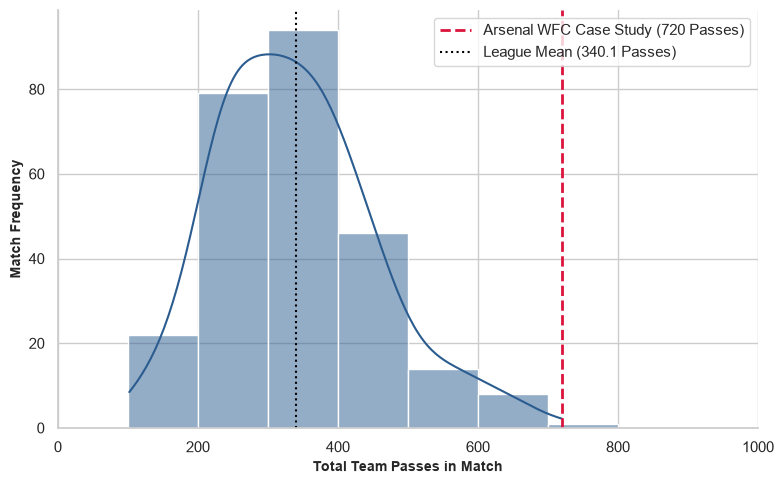
\includegraphics[width=0.85\textwidth]{figures/pass_histogram.png}
    \caption{League Match-Team Pass Distribution Histogram (WSL 2023/2024).}
    \label{fig:pass_histogram}
\end{figure}

% ==============================================================================
% 6. TRADITIONAL NULLS
% ==============================================================================
\newpage
\section{Traditional Nulls}
\label{sec:traditional_nulls}

Traditional null models face severe domain-specific deficiencies when applied to football. Generating a network null model involves randomizing topological features while preserving select global properties, such as total edge weight or node degree. However, football passing networks are constrained by physical pitch dimensions, player positioning, and tactical behavior. Traditional null models ignore these spatial and structural realities, generating unrealistic networks characterized by unnatural cross-field connections and misplaced playmaking hubs.

\subsection{Erd{\H{o}}s--R{\'e}nyi (ER) Random Model}
\label{subsec:er_model}

The simplest benchmarking approach is the Erd{\H{o}}s--R{\'e}nyi random graph framework, specifically the $G(N, p)$ model \cite{gilbert1959, erdos1959}. Under this formulation, $N$ nodes are connected independently with uniform probability $p$. For weighted passing networks, total pass volume ($720$ passes across $11$ nodes) is preserved, but topological structure is erased. Weights are distributed uniformly across all potential node pairs, treating all players as structural equals and discarding individual node degree constraints.

\subsection{Traditional Null Network Validation}
\label{subsec:null_validation}

Evaluating macro-level properties confirms that random edge generation fundamentally destroys realistic football network topology (\hyperref[tab:er_null_metrics]{Table~\ref{tab:er_null_metrics}}). In an Erd{\H{o}}s--R{\'e}nyi ($G(N, p)$) random model, uniform weight assignment erases operational workload inequality. Team Node Volume Variance collapses to $\text{Var}(s_{\text{tot}}) = 514.9917$ ($\sigma_{s_{\text{tot}}} \approx 22.69$ passes), homogeneously smoothing possession across all players and removing tactical playmaking hubs. Topologically, the PassMap degrades into an uninformative dense network where edge weights lack tactical variance and peripheral nodes erroneously appear as major distribution outlets.

This breakdown extends to downstream clustering. Global Mean Transitive Intensity artificially inflates ($\bar{I}_{\text{transitive}} = 708.54$), as uniform edge generation forces nearly every three-node combination into a dense cluster. Inspecting top active triads yields tactical impossibilities, such as high-capacity loops linking central forward Stina Blackstenius with defender Lotte Wubben-Moy ($69.0$ units) or goalkeeper Sabrina D’Angelo ($51.0$ units) (\hyperref[app:null_triad]{Appendix~\ref{app:null_triad}}). Plotting these triads (\hyperref[fig:er_null_failure]{Figure~\ref{fig:er_null_failure}}) produces non-local pitch-wide polygons, proving the spatial unviability of ER models for football networks.

\begin{table}[htbp]
    \centering
    \caption{ER Null Macro-Level Network Metrics vs. Empirical Sample}
    \label{tab:er_null_metrics}
    \begin{tabularx}{0.85\textwidth}{X c c c}
        \toprule
        \textbf{Metric} & \textbf{Notation} & \textbf{ER Null} & \textbf{Empirical} \\
        \midrule
        \textbf{Team Node Volume Variance} & $\text{Var}(s_{\text{tot}})$ & 514.9917 & 5681.9008 \\
        \textbf{Mean Unweighted Degree} & $\langle k \rangle$ & 15.4545 & 16.1818 \\
        \textbf{Degree Variance} & $\text{Var}(k)$ & 4.0661 & 7.7851 \\
        \textbf{Degree Standard Deviation} & $\sigma_k$ & 2.0165 & 2.7902 \\
        \textbf{Second Moment} & $\langle k^2 \rangle$ & 242.9091 & 269.6364 \\
        \textbf{Coefficient of Variation} & $CV_k$ & 0.1305 & 0.1724 \\
        \textbf{Normalized Second Moment} & $\langle k^2 \rangle / \langle k \rangle$ & 15.7176 & 16.6629 \\
        \bottomrule
    \end{tabularx}
\end{table}

\newpage
\begin{figure}[htbp]
    \centering
    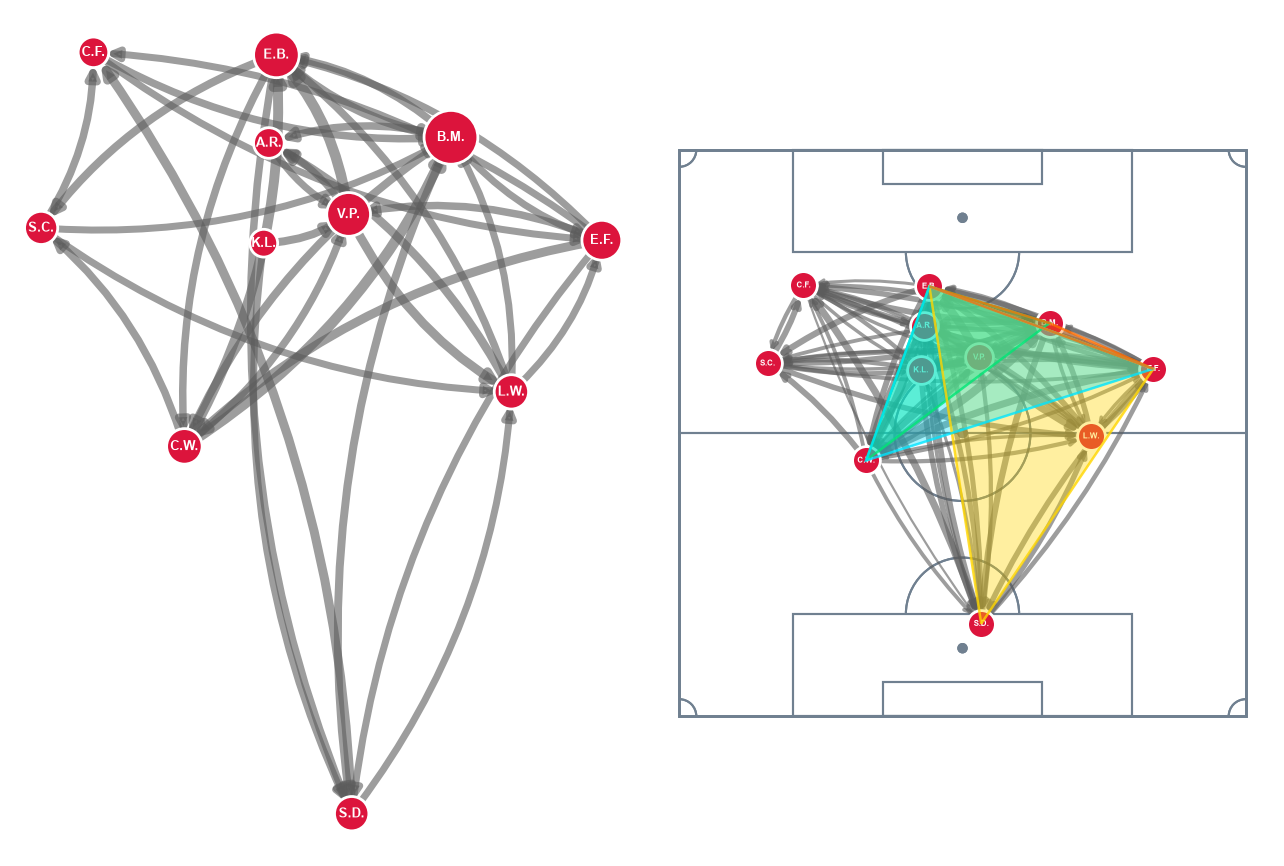
\includegraphics[width=0.9\textwidth]{figures/null_failure_network.png}
    \caption{ER Null Network Visual (Left) and ER Triad Network Plot (Right).}
    \label{fig:er_null_failure}
\end{figure}

% ==============================================================================
% 7. MARKOVIAN NULL MODEL
% ==============================================================================
\clearpage
\section{Markovian Null Model}
\label{sec:markovian_null}

The failure of naive, traditional null models necessitates a fundamental conceptual shift. A valid null model for football passing networks cannot treat the pitch as an abstract, unconstrained graph topology, it must strictly respect the spatial, physical, and tactical realities of match play.

\subsection{Markovian Processes and Stochastic Transformations}
\label{subsec:markovian_processes}

To construct a domain-aware generative baseline, we draw upon established football network literature modeling match dynamics using stochastic processes \cite{narizuka2014statistical, gama2026stoch} and repurpose the methodologies for null generation, shifting from modeling dynamics on a network to governing the dynamics of the network.

While existing literature predominantly applies Markov chains to fixed adjacency matrices to analyze possession diffusion, our generative task synthesizes entirely new reference network topologies ($\mathcal{G}_{\text{null}}$). We invert this paradigm by using learned spatial transition rules as a generative engine to resample synthetic pass events before aggregating the final null network.

This inversion addresses a critical research gap. Although stochastic flow models were originally used football network researchers to bypass traditional nulls, evaluating whether observed flow metrics reflect genuine tactical organization also ultimately requires benchmarking against a spatially constrained null ensemble \cite{gama2026stoch}.

\subsubsection{Justifying First-Order Markovian Processes}
\label{subsubsec:first_order_justification}

A first-order Markov process assumes that state transition probabilities ($X_{t+1}$) depend strictly on the current state ($X_t$):
\begin{equation}
    P(X_{t+1} = x \mid X_t = x_t, \dots, X_1 = x_1) = P(X_{t+1} = x \mid X_t = x_t)
\end{equation}

While higher-order memory is necessary for tracking sequential possession dynamics, a first-order memoryless formulation provides a parsimonious, mathematically aligned baseline for synthesizing static PassMap topologies. Standard $11 \times 11$ adjacency matrices aggregate full-match events statically, discarding temporal ordering. As a result, a first-order process provides the ideal structural fit for synthesizing these target networks. Furthermore, it has been demonstrated \cite{narizuka2014statistical} that a first-order spatial Markov process parameterised by distance decay successfully reproduces Small-World properties and truncated degree distributions without higher-order memory overhead.


\subsection{Domain Requirements \& Spatial Resampling Design}
\label{subsec:domain_resampling_design}

Buld{\'u} et al. \cite{buldu2018} emphasize that valid null models for football networks must maintain high domain realism by preserving physical game constraints, spatial player distributions, and pass length mechanics. To satisfy this, we propose a targeted spatial pass-recipient resampling model. Under this framework, each recorded pass's origin location, passer identity, and pitch phase are held fixed, while the recipient is systematically resampled using a first-order Markov process.

This design choice explicitly balances tactical destruction with domain validity. Retaining empirical match coordinates means actual positional occupancy zones and realistic pass-distance decay mechanics are not lost. Simultaneously, decoupling the original recipient breaks existing tactical systems and specific player-to-player relationships.

Finally, resampling recipients using spatial transition probabilities re-establishes network edges under strict physical constraints. This prevents structural anomalies, such as long-range goalkeeper-to-striker loops, while allowing central hubs to form naturally through emergent spatial proximity.

\subsection{Data Corpus Engineering}
\label{subsec:data_corpus_engineering}

Our generative resampling engine is parameterized across a large-scale league-wide dataset comprising $89,781$ completed passes from the 2023/2024 FA Women's Super League. Constructing the first-order Markovian model directly on raw passes---rather than finalized networks---ensures the resampling process inherently preserves spatial coordinates and physical game constraints.

Raw StatsBomb pitch coordinates ($120 \times 80$) are normalized to a standardized $100 \times 100$ scale and discretized into a $10 \times 10$ spatial grid of 100 uniform cells (\hyperref[fig:pitch_grid]{Figure~\ref{fig:pitch_grid}}). Granular player positions are mapped into a condensed positional taxonomy (\hyperref[app:cond_pos]{Appendix~\ref{app:cond_pos}}), eliminating team-specific lateral biases while retaining essential functional roles. This spatial and positional aggregation maximizes data density per pitch cell, enabling the Markovian transition model to learn robust, role-based spatial transition probabilities across the dataset.

\subsection{Recipient Probability Distribution Training}
\label{subsec:recipient_prob_training}

Using the discretized spatial grid and condensed positional taxonomy, we compile the pass data into a 3D Spatial Probability Tensor $\mathcal{P}$ of shape $(10, 10, N_{\text{pos}})$, where $N_{\text{pos}} = 9$. Each tensor element $\mathcal{P}(r, c, p)$ records pass frequencies terminating in cell $(r, c)$ received by position $p$. To prevent zero-probability artifacts in sparse pitch zones, we apply Laplace Additive Smoothing ($\alpha = 1.0$):
\begin{equation}
    \text{Counts}_{\text{smoothed}}(r, c, p) = \text{RawCount}(r, c, p) + 1.0
\end{equation}

Normalizing these smoothed counts yields the conditional recipient probability distribution $P(\text{Position } p \mid \text{Pass Ends in Bin } (r, c))$:
\begin{equation}
    P(p \mid r, c) = \frac{\text{Counts}_{\text{smoothed}}(r, c, p)}{\sum_{p'} \text{Counts}_{\text{smoothed}}(r, c, p')}
\end{equation}

This partitions the pitch into discrete spatial sectors governing recipient likelihood. For instance, central cell $(5,5)$ assigns highest reception probabilities to central midfielders ($38.96\%$) and central defenders ($30.58\%$), while goalkeeper receptions drop to $0.11\%$ (\hyperref[tab:spatial_recipient_prob_55]{Table~\ref{tab:spatial_recipient_prob_55}}). Sampling from these localized distributions ensures generated passes assign plausible recipients based on empirical behavior.

\newpage
\begin{figure}[H]
    \centering
    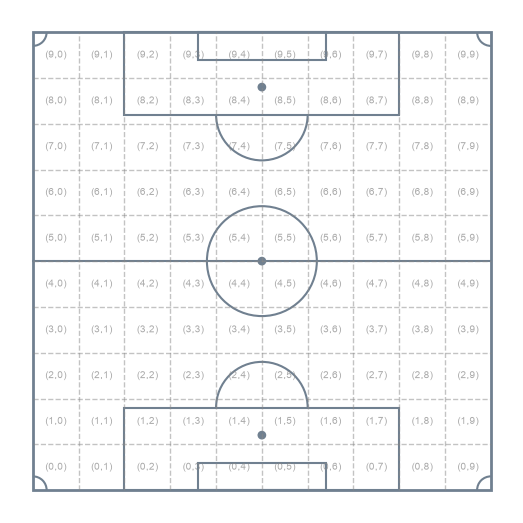
\includegraphics[height=0.60\textheight, keepaspectratio]{figures/pitch_grid.png}
    \caption{Pitch Plot Segmented into a $10 \times 10$ Spatial Grid.}
    \label{fig:pitch_grid}
\end{figure}

\vspace{0.5cm}

\begin{table}[H]
    \centering
    \small
    \caption{Spatial Recipient Probability Distribution for Pitch Bin $(5,5)$.}
    \label{tab:spatial_recipient_prob_55}
    \begin{tabularx}{0.75\textwidth}{c X c c}
        \toprule
        \textbf{Rank} & \textbf{Position} & \textbf{Probability} & \textbf{Probability (\%)} \\
        \midrule
        \textbf{1} & CM & 0.3896 & 38.96 \\
        \textbf{2} & CB & 0.3058 & 30.58 \\
        \textbf{3} & ST & 0.1143 & 11.43 \\
        \textbf{4} & RB & 0.0588 & 5.88 \\
        \textbf{5} & CAM & 0.0468 & 4.68 \\
        \textbf{6} & RM & 0.0305 & 3.05 \\
        \textbf{7} & LB & 0.0272 & 2.72 \\
        \textbf{8} & LM & 0.0261 & 2.61 \\
        \textbf{9} & GK & 0.0011 & 0.11 \\
        \bottomrule
    \end{tabularx}
\end{table}

\newpage
\subsection{Generative Markovian Recipient Resampling}
\label{subsec:markovian_resampling}

For each empirical pass in the target match, the engine retains the origin, end location, and passer identity (\hyperref[tab:sample_resampling_stream]{Table~\ref{tab:sample_resampling_stream}}). The terminal coordinates query the learned probability tensor $P(p \mid r, c)$ to sample a recipient position, which is mapped to an active teammate. Self-passes ($A \to A$) are strictly prevented. Exploring the resampled event stream prior to network aggregation confirms the engine successfully balances generative variance with domain realism (\hyperref[app:markovian_resampling_analysis]{Appendix~\ref{app:markovian_resampling_analysis}})

\begin{table}[htbp]
    \centering
    \small
    \caption{Sample Event Resampling and Player Mapping Stream.}
    \label{tab:sample_resampling_stream}
    \begin{tabularx}{\textwidth}{c X c c X X}
        \toprule
        \textbf{Pass ID} & \textbf{Passer (Origin)} & \textbf{Bin} & \textbf{Drawn Pos.} & \textbf{Empirical} & \textbf{Resampled} \\
        \midrule
        101 & W-Moy & (2, 4) & CB & Williamson & Williamson \\
        102 & Little & (5, 5) & CM & Pelova & Pelova \\
        103 & Catley & (7, 2) & LM & Foord & Foord \\
        104 & Pelova & (5, 8) & RB & Fox & Fox \\
        105 & W-Moy & (4, 5) & CM & Little & Pelova \\
        106 & Little & (8, 5) & ST & Russo & Blackstenius \\
        \bottomrule
    \end{tabularx}
\end{table}

\subsection{Sample Null Passing Network}
\label{subsec:sample_null_passing_network}

Visual comparison of the empirical network alongside a single null demonstrates that spatial recipient resampling produces a natural, pitch-constrained topology. Unlike the Erd{\H{o}}s--R{\'e}nyi model, the rewired graph avoids pitch-wide ``hairball'' artifacts while maintaining realistic player positioning and passing channels.

\begin{figure}[H]
    \centering
    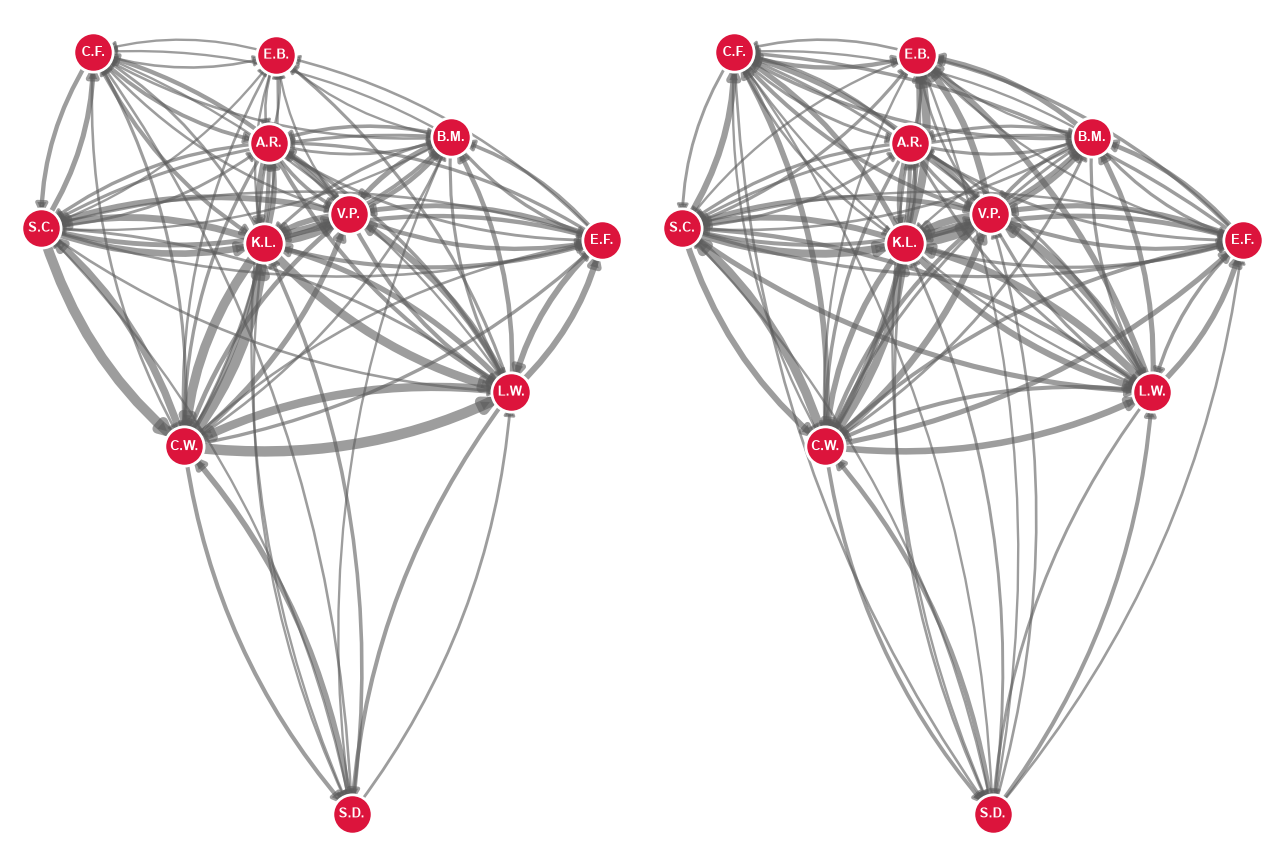
\includegraphics[width=0.55\textwidth]{figures/resample_orig_null.png}
    \caption{Empirical PassMap (Left) vs. Spatial Null Realization PassMap (Right).}
    \label{fig:resample_orig_null}
\end{figure}

\newpage
\subsubsection{Topological Degree Diagnostics}
\label{subsubsec:topological_degree_diagnostics}

Evaluating macro-level degree properties across this single realization confirms the spatial engine synthesizes domain-valid reference networks (\hyperref[tab:sample_null_metrics]{Table~\ref{tab:sample_null_metrics}}).

Holding passer volume ($s_i^{\text{out}}$) fixed recovers over half of empirical workload inequality ($\text{Var}(s_{\text{tot}}) = 2955.90$ vs. ER's $514.99$). This reveals passer initiative accounts for roughly $52\%$ of workload variance, while receiver choice drives $48\%$.

Replacing match-specific target preferences with league-average spatial probabilities increases active density ($\langle k \rangle = 17.64$) and flattens connection variance ($CV_k = 0.1115$). The Normalized Second Moment ($17.86$) closely tracks mean degree, proving empirical origin coordinates preserve structural density without creating scale-free hub anomalies.

\begin{table}[htbp]
    \centering
    \scriptsize
    \caption{Sample Null Macro-Level Metrics vs. Empirical and ER Baselines.}
    \label{tab:sample_null_metrics}
    \begin{tabularx}{0.85\textwidth}{X c c c}
        \toprule
        \textbf{Metric} & \textbf{Empirical} & \textbf{ER ($G(N,p)$)} & \textbf{Null} \\
        \midrule
        \textbf{Mean Unweighted Degree ($\langle k \rangle$)} & 16.1818 & 15.4545 & 17.6364 \\
        \addlinespace[3pt]
        \textbf{Coefficient of Variation ($CV_k$)} & 0.1724 & 0.1305 & 0.1115 \\
        \addlinespace[3pt]
        \textbf{Normalized Second Moment ($\frac{\langle k^2 \rangle}{\langle k \rangle}$)} & 16.6629 & 15.7176 & 17.8557 \\
        \addlinespace[3pt]
        \textbf{Node Volume Variance ($\text{Var}(s_{\text{tot}})$)} & 5681.90 & 514.99 & 2955.90 \\
        \bottomrule
    \end{tabularx}
\end{table}

\clearpage
\section{Null Validation}
\label{sec:null_validation}

While a single realization confirms local feasibility, formal validation requires a multi-run simulation to establish statistical stability and boundary constraints. Executing a 500-run Monte Carlo pipeline confirms that spatial recipient resampling reliably strips away match-specific tactical nuances across the entire null ensemble while strictly preserving domain-level topological invariants.

\subsection{Macro-Level Heterogeneity and Structural Density}
\label{subsec:macro_heterogeneity_density}

Across the 500-iteration ensemble, macro-level degree metrics confirm that spatial resampling maintains realistic structural density while suppressing extreme topological distortions (\hyperref[tab:null_validation_summary]{Table~\ref{tab:null_validation_summary}}). The Mean Unweighted Degree averages $\langle k \rangle = 17.7411$ ($95\%$ CI: $[16.9955, 18.3636]$), representing an expected connection density ($\approx 88.7\%$) that populates peripheral channels without exceeding pitch boundaries.

The Coefficient of Variation ($CV_k = 0.1196$) remains well below scale-free thresholds ($CV_k \ge 1.0$), while the empirical value ($0.1724$) sits above the upper confidence bound ($0.1615$), confirming match-specific tactical heterogeneity. Additionally, the Normalized Second Moment ($18.0011$) closely tracks mean degree, proving the ensemble operates within logical domain boundaries without generating central super-hubs.

\subsection{Workload Variance}
\label{subsec:workload_variance}

Holding passer volume ($s_i^{\text{out}}$) fixed allows the spatial model to recover over half of empirical workload inequality. The ensemble Team Node Volume Variance ($\text{Var}(s_{\text{tot}})$) averages $3117.38$ ($95\%$ CI: $[2672.08, 3629.00]$), capturing $55\%$ of empirical variance ($5681.90$). This establishes that passer initiative accounts for roughly $55\%$ of volume centralization, while targeted receiver selection drives $45\%$.

However, even the maximum simulated variance ($4000.45$) falls short of the empirical value. Although the null model reliably generates valid football network topologies, it struggles to reproduce the extreme tactical nuances present in our sample match. This is because averaging spatial probabilities across the league smooths out distinct operational profiles such as high overall possession with a low-touch striker as per this Arsenal team. Alternatively, this gap could simply reflect an undersampled Monte Carlo iteration space that has yet to hit the true distribution tail.

\subsection{Role Realism}
\label{subsec:role_realism}

Functional role realism is similarly preserved across all iterations. Goalkeeper Sabrina D’Angelo’s total pass volume stays tightly bounded with an ensemble mean of $43.2300$ passes ($95\%$ CI: $[38.0000, 49.0000]$) and a range of $[35.0, 51.0]$. Unlike Erd{\H{o}}s--R{\'e}nyi random graphs that erroneously transform the goalkeeper into an active playmaking hub, the spatial engine encodes positional constraints across every generated instance.

\subsection{Generative Matrix Variance}
\label{subsec:matrix_variance}

Evaluating the correlation between empirical and resampled weighted adjacency matrices yields an ensemble mean of $\bar{r} = 0.6753$ ($95\%$ CI: $[0.6026, 0.7468]$). This moderate-to-high correlation verifies that while the model preserves fundamental spatial structure and high-volume passing channels, it introduces sufficient generative variance to shuffle tactical nuances without collapsing into uncorrelated random noise or duplicating the input matrix.

\begin{table}[htbp]
    \centering
    \scriptsize
    \setlength{\tabcolsep}{3pt} % Reduces padding between columns
    \caption{Markovian Null Model Validation Summary ($N=500$ Iterations).}
    \label{tab:null_validation_summary}
    \begin{tabularx}{\textwidth}{X c c c c c c c}
        \toprule
        \textbf{Metric} & \textbf{Empirical} & \textbf{Null Mean} & \textbf{Null Std} & \textbf{Min} & \textbf{Max} & \textbf{95\% CI Low} & \textbf{95\% CI High} \\
        \midrule
        \textbf{Mean Degree ($\langle k \rangle$)} & 16.1818 & 17.7411 & 0.3923 & 16.7273 & 18.7273 & 16.9955 & 18.3636 \\
        \addlinespace[3pt]
        \textbf{Variation Coeff. ($CV_k$)} & 0.1724 & 0.1196 & 0.0209 & 0.0648 & 0.1755 & 0.0813 & 0.1615 \\
        \addlinespace[3pt]
        \textbf{Second Moment ($\frac{\langle k^2 \rangle}{\langle k \rangle}$)} & 16.6629 & 18.0011 & 0.3303 & 17.0978 & 18.8738 & 17.3529 & 18.5998 \\
        \addlinespace[3pt]
        \textbf{Node Var. ($\text{Var}(s_{\text{tot}})$)} & 5681.9008 & 3117.3808 & 246.0137 & 2382.2645 & 4000.4463 & 2672.0826 & 3629.0008 \\
        \addlinespace[3pt]
        \textbf{GK Volume ($s_{\text{tot}}$)} & 38.0000 & 43.2300 & 2.9443 & 35.0000 & 51.0000 & 38.0000 & 49.0000 \\
        \addlinespace[3pt]
        \textbf{Adjacency Corr. ($r$)} & 1.0000 & 0.6753 & 0.0377 & 0.5544 & 0.7678 & 0.6026 & 0.7468 \\
        \bottomrule
    \end{tabularx}
\end{table}

\clearpage
\section{Null-Baselined Metric Evaluation}
\label{sec:null_baselined_evaluation}

\subsection{Experimental Setup \& Simulation Scope}
\label{subsec:experimental_setup}

To evaluate empirical network properties against a spatially constrained baseline, we executed $N = 1000$ Markovian resampling iterations over the target match event stream, tracking the full suite of network metrics detailed in \hyperref[sec:metrics]{Section~\ref{sec:metrics}} across each run.

\subsection{Macro-Level Evaluation: Global Circulation Distance ($d$)}
\label{subsec:macro_evaluation}

Evaluating global average shortest path ($d = 0.1884$) against the 1000-iteration spatial null ensemble reveals that Arsenal WFC’s circulation efficiency emerges primarily from spatial territory and pass volume rather than unique tactics or elite performance (\hyperref[tab:null_macro_summary]{Table~\ref{tab:null_macro_summary}}).

The empirical path length sits slightly below the null mean ($\bar{d}_{\text{null}} = 0.1932$, $z = -0.43$) but well within the $95\%$ confidence interval ($[0.1732, 0.2120]$). Completing over 700 passes inherently dictates the global distance. One reason Arsenal's path length remains above the theoretical minimum ($0.1732$) is because they forgo global efficiency in lieu of deliberate, localized tactical overloads.

\begin{table}[htbp]
    \centering
    \scriptsize
    \caption{Null-Baselined Macro Evaluation Summary}
    \label{tab:null_macro_summary}
    \begin{tabularx}{0.85\textwidth}{l l c c c c}
        \toprule
        \textbf{Scale} & \textbf{Metric} & \textbf{Empirical} & \textbf{Null Mean} & \textbf{Null 95\% CI} & \textbf{$Z$-Score} \\
        \midrule
        \textbf{Macro} & Global Shortest Path ($d$) & 0.1884 & 0.1932 & [0.1732, 0.2120] & $-0.43$ \\
        \bottomrule
    \end{tabularx}
\end{table}

\subsection{Meso-Level Evaluation: Transitive Triad Dynamics ($I_{\text{transitive}}$)}
\label{subsec:meso_evaluation}

Benchmarking the top 20 empirical transitive triads against the 1,000-iteration spatial null ensemble separates intentional tactical mechanics from simple spatial occupancy (\hyperref[tab:null_meso_summary]{Table~\ref{tab:null_meso_summary}}).

Deep build-up triangles demonstrate extreme statistical significance. The rank 1 triad (W.Moy--Little--Williamson; $116.00$ units, $z = +3.83$) and rank 2 left-flank triangle (W.Moy--Little--Catley; $111.00$ units, $z = +5.67$) comfortably exceed null $95\%$ upper bounds ($98.00$ and $78.00$, respectively), confirming an intentional left-sided overloading mechanism for progressive build-up.

Conversely, central recycling loops operate directly in line with spatial expectations. Triads like W.Moy--Little--Pelova ($69.00$ units, $z = -0.28$) track null means ($\bar{W} = 71.53$) almost perfectly, proving their high volume reflects spatial density rather than specialized tactics.

Finally, Alessia Russo’s participation across progressive triads consistently surpasses null bounds ($z$-scores between $+1.84$ and $+2.78$), proving her deep-dropping movement represents deliberate tactical linkage rather than spatial chance.

\subsection{Micro-Level Evaluation: Positional Betweenness Centrality ($g(i)$)}
\label{subsec:micro_evaluation}

Evaluating empirical betweenness centrality ($g(i)$) against the 1,000-iteration spatial null baseline reveals how Arsenal WFC explicitly structures its build-up play (\hyperref[tab:null_micro_summary]{Table~\ref{tab:null_micro_summary}}).

The central defensive core operates as a primary routing engine: both Left Center Back ($g = 0.3222, z = +2.73$) and Right Center Back ($g = 0.3000, z = +2.85$) exceed their upper $95\%$ confidence bounds ($0.2668$ and $0.2556$), proving their central conduit role is an explicit tactical instruction.

Controlling for empirical spatial pass volume reveals a clear left-flank asymmetry in Arsenal's network. Left Back Steph Catley operates near the upper limit of her spatial expectation ($g = 0.1222, z = +1.73$ against a $[0.0000, 0.1556]$ baseline), whereas the Right Back registers zero betweenness ($g = 0.0000$). Conversely, the Left Defensive Midfield falls below its spatial baseline ($\bar{g} = 0.2896$ vs. $g = 0.1778, z = -1.31$), demonstrating that Arsenal avoids over-funneling progression through a single central pivot.

\begin{table}[htbp]
    \centering
    \scriptsize
    \setlength{\tabcolsep}{3pt} % Reduces padding between columns
    \caption{Null-Baselined Meso Evaluation Summary}
    \label{tab:null_meso_summary}
    \begin{tabularx}{\textwidth}{c X c c c c}
        \toprule
        \textbf{Rank} & \textbf{Targeted Triad ($A - B - C$)} & \textbf{Empirical} & \textbf{Null Mean} & \textbf{Null 95\% CI} & \textbf{$Z$-Score} \\
        \midrule
        1  & Wubben-Moy---\allowbreak Little---\allowbreak Williamson & 116.00 & 79.23 & [61.00, 98.00] & $+3.83$ \\
        2  & Wubben-Moy---\allowbreak Little---\allowbreak Catley     & 111.00 & 61.11 & [44.00, 78.00] & $+5.67$ \\
        3  & Little---\allowbreak Catley---\allowbreak Pelova         & 76.00  & 56.74 & [39.00, 74.00] & $+2.11$ \\
        4  & Wubben-Moy---\allowbreak Little---\allowbreak Pelova     & 69.00  & 71.53 & [54.98, 89.00] & $-0.28$ \\
        5  & Little---\allowbreak Williamson---\allowbreak Pelova     & 67.00  & 66.89 & [50.00, 85.00] & $+0.01$ \\
        6  & Wubben-Moy---\allowbreak Catley---\allowbreak Pelova     & 65.00  & 49.48 & [34.00, 65.00] & $+1.97$ \\
        7  & Wubben-Moy---\allowbreak Williamson---\allowbreak Pelova & 60.00  & 57.81 & [42.00, 73.00] & $+0.28$ \\
        8  & Fox---\allowbreak Williamson---\allowbreak Pelova        & 55.00  & 37.90 & [24.00, 52.00] & $+2.47$ \\
        9  & Russo---\allowbreak Little---\allowbreak Pelova          & 51.00  & 36.34 & [21.00, 51.00] & $+1.87$ \\
        10 & Fox---\allowbreak Little---\allowbreak Pelova            & 51.00  & 40.84 & [25.00, 57.00] & $+1.30$ \\
        11 & Fox---\allowbreak Little---\allowbreak Williamson        & 51.00  & 38.20 & [23.00, 54.00] & $+1.63$ \\
        12 & Russo---\allowbreak Little---\allowbreak Williamson      & 42.00  & 24.05 & [10.00, 39.00] & $+2.44$ \\
        13 & Mead---\allowbreak Williamson---\allowbreak Pelova       & 40.00  & 25.52 & [15.00, 37.02] & $+2.44$ \\
        14 & Russo---\allowbreak Wubben-Moy---\allowbreak Little      & 39.00  & 25.58 & [12.00, 40.00] & $+1.84$ \\
        15 & Russo---\allowbreak Williamson---\allowbreak Pelova      & 38.00  & 22.44 & [9.00, 36.00]  & $+2.30$ \\
        16 & Russo---\allowbreak Wubben-Moy---\allowbreak Pelova      & 37.00  & 23.67 & [11.00, 37.00] & $+2.00$ \\
        17 & Russo---\allowbreak Wubben-Moy---\allowbreak Williamson  & 35.00  & 18.79 & [7.00, 30.00]  & $+2.78$ \\
        18 & Foord---\allowbreak Little---\allowbreak Catley          & 33.00  & 37.36 & [25.00, 50.00] & $-0.67$ \\
        19 & Foord---\allowbreak Catley---\allowbreak Pelova          & 33.00  & 32.95 & [21.00, 45.00] & $+0.01$ \\
        20 & Wubben-Moy---\allowbreak Williamson---\allowbreak D’Angelo & 33.00 & 32.70 & [21.00, 44.02] & $+0.05$ \\
        \bottomrule
    \end{tabularx}
\end{table}


\begin{table}[htbp]
    \centering
    \scriptsize
    \setlength{\tabcolsep}{3pt} % Reduces padding between columns
    \caption{Null-Baselined Micro Evaluation Summary}
    \label{tab:null_micro_summary}
    \begin{tabularx}{\textwidth}{X c c c c}
        \toprule
        \textbf{Targeted Position} & \textbf{Empirical} & \textbf{Null Mean} & \textbf{Null 95\% CI} & \textbf{$Z$-Score} \\
        \midrule
        Betweenness: Left Center Back & 0.3222 & 0.1471 & [0.0222, 0.2668] & $+2.73$ \\
        Betweenness: Right Center Back & 0.3000 & 0.1149 & [0.0111, 0.2556] & $+2.85$ \\
        Betweenness: Left Back & 0.1222 & 0.0426 & [0.0000, 0.1556] & $+1.73$ \\
        Betweenness: Right Defensive Midfield & 0.1389 & 0.1367 & [0.0111, 0.2778] & $+0.03$ \\
        Betweenness: Left Defensive Midfield & 0.1778 & 0.2896 & [0.1313, 0.4556] & $-1.31$ \\
        Betweenness: Right Back & 0.0000 & 0.0071 & [0.0000, 0.0667] & $-0.38$ \\
        Betweenness: Left Wing & 0.0000 & 0.0058 & [0.0000, 0.1000] & $-0.27$ \\
        Betweenness: Right Wing & 0.0000 & 0.0054 & [0.0000, 0.1000] & $-0.27$ \\
        Betweenness: Center Attacking Midfield & 0.0000 & 0.0038 & [0.0000, 0.0889] & $-0.22$ \\
        Betweenness: Goalkeeper & 0.0000 & 0.0001 & [0.0000, 0.0000] & $-0.03$ \\
        Betweenness: Center Forward & 0.0000 & 0.0000 & [0.0000, 0.0000] & $0.00$ \\
        \bottomrule
    \end{tabularx}
\end{table}

\clearpage
\section{Conclusion, Limitations, and Future Work}
\label{sec:conclusion_limitations_future}

\subsection{Conclusion}
\label{subsec:conclusion}

This paper demonstrates the intersection of network science and sports analytics, evaluating collective tactical behavior in football through network properties. By leveraging open-source StatsBomb event data from the 2023/2024 FA Women's Super League, this research converted raw spatiotemporal events into directed, weighted PassMaps, addressing the systemic underrepresentation of women's football in quantitative literature.

The project deployed a multi-scale diagnostic suite across micro (betweenness centrality), meso (transitive triads), and macro (global shortest paths) graph dimensions, supported by custom spatial visualization tools.

This research directly responds to calls in the literature \cite{gama2026stoch} for robust null baselines. We validated that traditional randomizations, such as Erd{\H{o}}s--R{\'e}nyi, fail in this domain by destroying pitch geometry, flattening workload inequality, and generating structural role anomalies.

In response, we engineered a novel first-order Spatial Markovian generative null process. Inverting the analytical lens from state dynamics \textit{on} the network to generative dynamics \textit{of} the network, the engine resamples pass recipients using league-average spatial probabilities while strictly preserving empirical origin coordinates, passer identities, and physical pitch boundaries to ensure domain suitability.

Ultimately, executing this Monte Carlo null pipeline against an extreme high-volume match separated baseline geometric inevitabilities from deliberate tactical architecture, isolating true tactical signals—such as left-flank overloads and center-back redistribution—from spatial noise.

\subsection{Limitations}
\label{subsec:limitations}

While effective for synthesizing static PassMaps, the first-order Markovian framework carries two primary structural limitations. 

First, its memoryless assumption evaluates passes in isolation based purely on terminal spatial coordinates. By ignoring sequential, multi-step player interactions, the model washes out localized dynamics and complex combinational routines, which restricts higher-order triad analysis. 

Second, the framework lacks temporal and game-state context. Aggregating pass totals across full 90-minute matches ignores time elapsed and scoreline dynamics, such as chasing a late deficit versus early-game consolidation. Consequently, resampled recipients reflect broad spatial averages rather than the specific tactical context of the original pass.

\subsection{Future Work}
\label{subsec:future_work}

Future research should expand the null validation framework by establishing algorithmic bounds that dynamically adjust for tactical formations, team quality, and game states. 

Expanding the generative engine requires integrating temporal context, higher-order sequence memory, and multi-step player interactions to better reflect localized combination play. 

Additionally, broadening the generative scope beyond pass recipient to resample pass destinations and origins based on role constraints would enable full synthetic event-stream generation. Ensembling these steps will allow analysts to systematically benchmark passer initiative, decision-making, and systemic ball progression across any tactical scenario.










% ==============================================================================
% BIBLIOGRAPHY
% ==============================================================================

\newpage
\bibliographystyle{vancouver}
\bibliography{references}

% % ====================================
% % APPENDIX
% % ====================================
\clearpage
\appendix
\section*{Appendices}
\addcontentsline{toc}{section}{Appendices} % Adds "Appendices" to Table of Contents

% ------------------------------------------------------------------------------
% APPENDIX A: FOOTBALL NETWORK METRICS TAXONOMY
% ------------------------------------------------------------------------------
\section{Football Network Metrics Taxonomy}
\label{app:network_metrics_taxonomy}

\begin{table}[htbp]
    \centering
    \small
    \caption{Micro-Scale Network Metrics and Football Interpretations \cite{gama2026stoch}.}
    \label{tab:gama_micro_metrics}
    \begin{tabularx}{\textwidth}{l X}
        \toprule
        \textbf{Metric} & \textbf{Footballing Interpretation \& Tactical Meaning} \\
        \midrule
        \textbf{Degree Centrality} & \textbf{Volume of Direct Involvement:} Quantifies how frequently a player acts as a passer/receiver, indicating workload in possession circulation and immediate availability as an outlet. High values suggest greater involvement in ball circulation. \\
        \addlinespace[3pt]
        \textbf{Closeness Centrality} & \textbf{Distribution Speed:} Assesses how quickly a player can reach (or be reached by) teammates. Lower values suggest the ability to receive and distribute under time pressure; higher values may indicate peripheral positioning. \\
        \addlinespace[3pt]
        \textbf{Stress Centrality} & \textbf{Transitional Load:} Identifies players who bear the highest volume of passing traffic between sectors, indicating responsibility in maintaining possession during phase transitions. \\
        \addlinespace[3pt]
        \textbf{Betweenness Centrality} & \textbf{Connective Mediation:} Identifies players who bridge different team sectors (defense--midfield--attack), enabling transitions and bypassing opposition pressure. High values indicate an essential role in team structural connectivity. \\
        \addlinespace[3pt]
        \textbf{Degree Prestige} & \textbf{Solicited Player Target:} Identifies players who are most sought out by teammates during the game, as measured by the number of passes received. High values indicate trusted targets in possession. \\
        \addlinespace[3pt]
        \textbf{Eigenvector Centrality} & \textbf{Influence via Central Hubs:} Measures player importance based on being connected to other highly active, central players rather than just raw volume. High values denote key links within primary tactical cores. \\
        \addlinespace[3pt]
        \textbf{PageRank Centrality} & \textbf{Tactical Reference Point:} Identifies players who receive passes due to their perceived importance and positional quality. High values suggest teammates actively seek them out as reliable options under pressure. \\
        \addlinespace[3pt]
        \textbf{Clustering Coefficient} & \textbf{Local Combination Play:} Identifies players who favor quick passing exchanges in tight spaces. High values indicate participation in short, repetitive passing patterns. \\
        \bottomrule
    \end{tabularx}
\end{table}

% ==============================================================================
% APPENDIX TABLE 2: MACRO-SCALE NETWORK METRICS
% ==============================================================================
\newpage
\begin{table}[htbp]
    \centering
    \small
    \caption{Macro-Scale Network Metrics and Football Interpretations \cite{gama2026stoch}.}
    \label{tab:gama_macro_metrics}
    \begin{tabularx}{\textwidth}{l X}
        \toprule
        \textbf{Metric} & \textbf{Footballing Interpretation \& Tactical Meaning} \\
        \midrule
        \textbf{Total Links} & \textbf{Collective Involvement:} Total number of connected player pairs. Reflects overall team participation in possession and interaction diversity. \\
        \addlinespace[3pt]
        \textbf{Network Density} & \textbf{Interaction Fluidity:} Proportion of possible connections realized. Higher density suggests quick passing options and supported play; lower density indicates spatial dispersion or structured width. \\
        \addlinespace[3pt]
        \textbf{Average Distance} & \textbf{Structural Proximity:} Average path length between players. Shorter distances indicate tight positioning and quick exchange potential; longer distances suggest tactical width or isolated sectors. \\
        \addlinespace[3pt]
        \textbf{Network Diameter} & \textbf{Maximum Reorganization Length:} Longest shortest path between any two players. Indicates how quickly the team can reorganize possession across extremes of the formation. \\
        \addlinespace[3pt]
        \textbf{Network Heterogeneity} & \textbf{Interaction Concentration:} Measures variance in overall player involvement. High values indicate heavy concentration around a few core players; low values suggest balanced team distribution. \\
        \addlinespace[3pt]
        \textbf{Transitivity} & \textbf{Triangulation Tendency:} Measures the proportion of triplet connections that form closed triangles. Reflects capacity for quick passing combinations and small-group play. \\
        \addlinespace[3pt]
        \textbf{Reciprocity} & \textbf{Bidirectional Exchange:} Shows balance in two-way passing between player pairs. High reciprocity suggests mutual trust and balanced distribution; low reciprocity indicates directed, progression-oriented play. \\
        \addlinespace[3pt]
        \textbf{Global Centralization} & \textbf{Hub Dependence:} Indicates whether the team relies heavily on one or a few key players to conduct play. Higher values suggest tactical vulnerability if central hubs are marked out. \\
        \addlinespace[3pt]
        \textbf{Assortativity Coefficient} & \textbf{Role-Based Connectivity:} Identifies whether players tend to connect with similar or different positional roles. Negative values suggest functional integration across lines; positive values indicate within-role clustering. \\
        \bottomrule
    \end{tabularx}
\end{table}


% ------------------------------------------------------------------------------
% APPENDIX B: SAMPLE NETWORK BETWEENNESS CENTRALITY VALUES
% ------------------------------------------------------------------------------
\clearpage
\section{Sample Network Betweenness Centrality Scores}
\label{app:sample_betweenness_scores}

\begin{table}[htbp]
    \centering
    \small
    \caption{Sample Network Player Betweenness Centrality ($g(i)$) Scores.}
    \label{tab:app_sample_betweenness}
    \begin{tabularx}{0.85\textwidth}{X l c}
        \toprule
        \textbf{Player} & \textbf{Position} & \textbf{Betweenness Centrality $g(i)$} \\
        \midrule
        Carlotte Wubben-Moy & Left Center Back & 0.3222 \\
        Leah Williamson & Right Center Back & 0.3000 \\
        Kim Little & Left Defensive Midfield & 0.1778 \\
        Victoria Pelova & Right Defensive Midfield & 0.1389 \\
        Stephanie-Elise Catley & Left Back & 0.1222 \\
        Sabrina D’Angelo & Goalkeeper & 0.0000 \\
        Emma Stina Blackstenius & Center Forward & 0.0000 \\
        Alessia Russo & Center Attacking Midfield & 0.0000 \\
        Emily Ann Fox & Right Back & 0.0000 \\
        Caitlin Jade Foord & Left Wing & 0.0000 \\
        Bethany Mead & Right Wing & 0.0000 \\
        \bottomrule
    \end{tabularx}
\end{table}


% ------------------------------------------------------------------------------
% APPENDIX C: EMPIRICAL TRANSITIVE TRIADS
% ------------------------------------------------------------------------------
\clearpage
\section{Top Empirical Transitive Passing Triads}
\label{app:empirical_triads}

\begin{table}[htbp]
    \centering
    \small
    \caption{Top 10 Active Transitive Passing Triads (Sample Network).}
    \label{tab:app_empirical_triads}
    \begin{tabularx}{\textwidth}{c X X X c}
        \toprule
        \textbf{Rank} & \textbf{Origin / Target ($A$)} & \textbf{Intermediate ($B$)} & \textbf{Target / Origin ($C$)} & \textbf{Capacity ($W_{\text{min}}$)} \\
        \midrule
        \textbf{1} & Kim Little & Carlotte Wubben-Moy & Leah Williamson & 116.0 \\
        \textbf{2} & Stephanie-Elise Catley & Kim Little & Carlotte Wubben-Moy & 111.0 \\
        \textbf{3} & Stephanie-Elise Catley & Kim Little & Victoria Pelova & 76.0 \\
        \textbf{4} & Kim Little & Carlotte Wubben-Moy & Victoria Pelova & 69.0 \\
        \textbf{5} & Kim Little & Victoria Pelova & Leah Williamson & 67.0 \\
        \textbf{6} & Stephanie-Elise Catley & Carlotte Wubben-Moy & Victoria Pelova & 65.0 \\
        \textbf{7} & Carlotte Wubben-Moy & Victoria Pelova & Leah Williamson & 60.0 \\
        \textbf{8} & Victoria Pelova & Leah Williamson & Emily Ann Fox & 55.0 \\
        \textbf{9} & Kim Little & Alessia Russo & Victoria Pelova & 51.0 \\
        \textbf{10} & Kim Little & Victoria Pelova & Emily Ann Fox & 51.0 \\
        \bottomrule
    \end{tabularx}
\end{table}


% ------------------------------------------------------------------------------
% APPENDIX D: DATASET & POSITIONAL TAXONOMY
% ------------------------------------------------------------------------------
\clearpage
\section{Dataset and Positional Taxonomy}
\label{app:positional_taxonomy}

\begin{table}[htbp]
    \centering
    \small
    \caption{Distribution of Formations (200--299 Passes, $n = 94$)}
    \label{tab:formation_binning}
    \begin{tabularx}{0.7\textwidth}{X c c}
        \toprule
        \textbf{Formation} & \textbf{Match Count ($n$)} & \textbf{Percentage (\%)} \\
        \midrule
        \textbf{4-2-3-1} & 29 & 30.85 \\
        \textbf{3-5-2} & 14 & 14.89 \\
        \textbf{4-3-3} & 12 & 12.77 \\
        \textbf{4-1-4-1} & 11 & 11.70 \\
        \textbf{3-4-3} & 11 & 11.70 \\
        \textbf{4-4-2} & 6 & 6.38 \\
        \textbf{4-4-1-1} & 5 & 5.32 \\
        \textbf{3-4-1-2} & 3 & 3.19 \\
        \textbf{3-4-2-1} & 1 & 1.06 \\
        \textbf{4-1-2-1-2} & 1 & 1.06 \\
        \textbf{4-5-1} & 1 & 1.06 \\
        \bottomrule
    \end{tabularx}
\end{table}

% ------------------------------------------------------------------------------
% APPENDIX E: NULL TRIAD EVALUATION
% ------------------------------------------------------------------------------
\clearpage
\section{Null Model Triad Evaluation}
\label{app:null_triad}

\begin{table}[htbp]
    \centering
    \small
    \caption{Top 10 Active Transitive Triads (Erd{\H{o}}s--R{\'e}nyi Null Model).}
    \label{tab:er_null_triads}
    \begin{tabularx}{\textwidth}{c X X X c}
        \toprule
        \textbf{Rank} & \textbf{Origin ($A$)} & \textbf{Middle ($B$)} & \textbf{Target ($C$)} & \textbf{Value ($W_{\text{min}}$)} \\
        \midrule
        \textbf{1} & Blackstenius & Wubben-Moy & Mead & 69.0 \\
        \textbf{2} & D’Angelo & Blackstenius & Fox & 51.0 \\
        \textbf{3} & Blackstenius & Wubben-Moy & Fox & 46.0 \\
        \textbf{4} & Blackstenius & Fox & Mead & 44.0 \\
        \textbf{5} & Fox & Foord & Mead & 44.0 \\
        \textbf{6} & Catley & Foord & Mead & 43.0 \\
        \textbf{7} & Catley & Little & Mead & 42.0 \\
        \textbf{8} & Catley & Fox & Foord & 41.0 \\
        \textbf{9} & Wubben-Moy & Fox & Mead & 40.0 \\
        \textbf{10} & Little & Pelova & Mead & 39.0 \\
        \bottomrule
    \end{tabularx}
\end{table}



% ------------------------------------------------------------------------------
% APPENDIX F: CONDENSED POSITIONAL TAXONOMY AND MAPPING LOGIC
% ------------------------------------------------------------------------------
\clearpage
\section{Condensed Positional Taxonomy and Mapping Logical}
\label{app:cond_pos}

\begin{table}[htbp]
    \centering
    \small
    \caption{Condensed Position Categories with Original and Pass Volume.}
    \label{tab:condensed_positions_mapped}
    \begin{tabularx}{\textwidth}{c l X c}
        \toprule
        \textbf{Rank} & \textbf{Position} & \textbf{Original Position(s)} & \textbf{Pass Count} \\
        \midrule
        \textbf{1} & CB & Center Back, Left Center Back, Right Center Back & 25,544 \\
        \addlinespace[3pt]
        \textbf{2} & CM & Left Defensive Midfield, Center Defensive Midfield, Right Defensive Midfield, Left Center Midfield, Right Center Midfield & 20,027 \\
        \addlinespace[3pt]
        \textbf{3} & LB & Left Back, Left Wing Back & 8,554 \\
        \addlinespace[3pt]
        \textbf{4} & RB & Right Back, Right Wing Back & 8,003 \\
        \addlinespace[3pt]
        \textbf{5} & ST & Center Forward, Left Center Forward, Right Center Forward & 7,066 \\
        \addlinespace[3pt]
        \textbf{6} & GK & Goalkeeper & 6,730 \\
        \addlinespace[3pt]
        \textbf{7} & LM & Left Wing, Left Midfield & 5,461 \\
        \addlinespace[3pt]
        \textbf{8} & RM & Right Wing, Right Midfield & 5,256 \\
        \addlinespace[3pt]
        \textbf{9} & CAM & Center Attacking Midfield, Left Attacking Midfield, Right Attacking Midfield & 3,140 \\
        \bottomrule
    \end{tabularx}
\end{table}

% ------------------------------------------------------------------------------
% APPENDIX G: ORIGINAL GRANULAR POSITION COUNTS
% ------------------------------------------------------------------------------
\clearpage
\section{Original Position Counts}
\label{app:pos_count}

\begin{table}[htbp]
    \centering
    \small
    \caption{Original Granular Position Counts Across Season Corpus.}
    \label{tab:original_position_counts}
    \begin{tabularx}{0.75\textwidth}{c X c}
        \toprule
        \textbf{Index} & \textbf{Original Recipient Position} & \textbf{Count} \\
        \midrule
        0  & Left Center Back & 11,956 \\
        1  & Right Center Back & 10,913 \\
        2  & Goalkeeper & 6,730 \\
        3  & Left Back & 6,283 \\
        4  & Right Back & 5,926 \\
        5  & Left Defensive Midfield & 5,446 \\
        6  & Right Defensive Midfield & 4,997 \\
        7  & Center Forward & 4,469 \\
        8  & Left Wing & 4,315 \\
        9  & Right Wing & 4,103 \\
        10 & Center Defensive Midfield & 3,532 \\
        11 & Left Center Midfield & 3,065 \\
        12 & Right Center Midfield & 2,987 \\
        13 & Center Attacking Midfield & 2,729 \\
        14 & Center Back & 2,675 \\
        15 & Left Wing Back & 2,271 \\
        16 & Right Wing Back & 2,077 \\
        17 & Left Center Forward & 1,349 \\
        18 & Right Center Forward & 1,248 \\
        19 & Right Midfield & 1,153 \\
        20 & Left Midfield & 1,146 \\
        21 & Right Attacking Midfield & 213 \\
        22 & Left Attacking Midfield & 198 \\
        \bottomrule
    \end{tabularx}
\end{table}

% ------------------------------------------------------------------------------
% APPENDIX H: EMPIRICAL VS. RESAMPLED PASS SHARE
% ------------------------------------------------------------------------------
\clearpage
\section{Resampled Player Pass Share}
\label{app:pass_share}


\begin{table}[htbp]
    \centering
    \small
    \caption{Change in Pass Share: Empirical vs. Resampled Receptions.}
    \label{tab:pass_share_comparison}
    \begin{tabularx}{\textwidth}{X c c c c}
        \toprule
        \textbf{Player} & \textbf{Count} & \textbf{Share (\%)} & \textbf{Resampled Count} & \textbf{Resampled Share (\%)} \\
        \midrule
        Moy & 120 & 16.67 & 67 & 9.31 \\
        Little & 117 & 16.25 & 106 & 14.72 \\
        Williamson & 99 & 13.75 & 66 & 9.17 \\
        Pelova & 92 & 12.78 & 108 & 15.00 \\
        Catley & 79 & 10.97 & 70 & 9.72 \\
        Russo & 60 & 8.33 & 25 & 3.47 \\
        Fox & 48 & 6.67 & 48 & 6.67 \\
        Mead & 42 & 5.83 & 55 & 7.64 \\
        Foord & 33 & 4.58 & 65 & 9.03 \\
        D’Angelo & 19 & 2.64 & 14 & 1.94 \\
        Blackstenius & 11 & 1.53 & 96 & 13.33 \\
        \bottomrule
    \end{tabularx}
\end{table}


% ==============================================================================
% APPENDIX I: SENSE CHECKING THE RESAMPLED RECIPIENT DATASET
% ==============================================================================
\clearpage
\begin{samepage}
\section{Sense Checking the Resampled Recipient Dataset}
\label{app:markovian_resampling_analysis}

Evaluating the pre-aggregation resampled event stream confirms the engine balances generative variance with domain realism. Remapping $22.08\%$ of passes to their exact empirical recipient shows the model preserves localized spatial dominance without simply reproducing the input network. 

The framework enforces role boundaries—constraining goalkeeper Sabrina D’Angelo to 13 receptions (down from 19)—while highlighting structural trade-offs. Wingers Caitlin Foord and Beth Mead receive inflated pass shares because the model lacks temporal substitution weighting, treating their 63-minute appearances as full matches. 

Striker Stina Blackstenius shows the largest shift, rising from 11 empirical receptions ($1.53\%$) to 96 resampled receptions ($13.33\%$). Because Arsenal dominated deep territory where tensor bins assign high baseline probabilities to central forwards, this spike reflects territorial volume replacing her specialized off-ball isolation, rather than a generative failure (\hyperref[fig:striker_resample_plot]{Figure~\ref{fig:striker_resample_plot}}).

\begin{figure}[H]
    \centering
    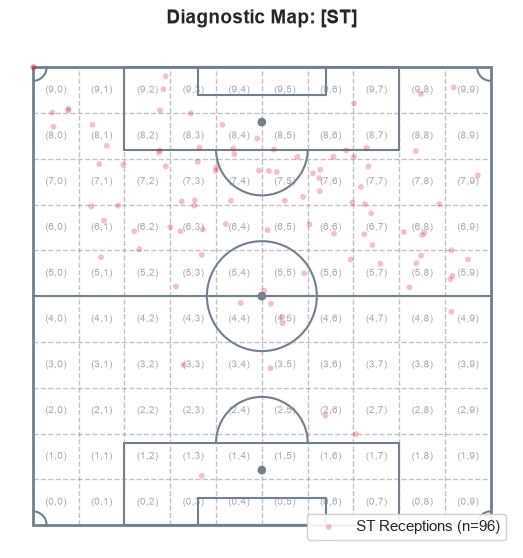
\includegraphics[width=0.75\textwidth]{figures/striker_resample_plot.png}
    \caption{Resampled Striker Reception Pitch Plot}
    \label{fig:striker_resample_plot}
\end{figure}
\end{samepage}

% ------------------------------------------------------------------------------
% APPENDIX J: LEAGUE-WIDE STRIKER PASS SUMMARY
% ------------------------------------------------------------------------------
\clearpage
\section{League Wide Striker Pass Summary}
\label{app:striker_pass}


\begin{table}[htbp]
    \centering
    \small
    \caption{League-Wide Striker Pass Execution Summary.}
    \label{tab:league_striker_summary}
    \begin{tabularx}{0.75\textwidth}{X c}
        \toprule
        \textbf{Metric} & \textbf{Value} \\
        \midrule
        \textbf{Total Completed Passes} & 89,781 \\
        \textbf{Striker Completed Passes} & 4,433 \\
        \textbf{Percentage Completed by Strikers} & 4.94\% \\
        \bottomrule
    \end{tabularx}
\end{table}



\end{document}